%% BioMed_Central_Tex_Template_v1.06
%%                                      %
%  bmc_article.tex            ver: 1.06 %
%                                       %

%%IMPORTANT: do not delete the first line of this template
%%It must be present to enable the BMC Submission system to
%%recognise this template!!

%%%%%%%%%%%%%%%%%%%%%%%%%%%%%%%%%%%%%%%%%
%%                                     %%
%%  LaTeX template for BioMed Central  %%
%%     journal article submissions     %%
%%                                     %%
%%          <8 June 2012>              %%
%%                                     %%
%%                                     %%
%%%%%%%%%%%%%%%%%%%%%%%%%%%%%%%%%%%%%%%%%


%%%%%%%%%%%%%%%%%%%%%%%%%%%%%%%%%%%%%%%%%%%%%%%%%%%%%%%%%%%%%%%%%%%%%
%%                                                                 %%
%% For instructions on how to fill out this Tex template           %%
%% document please refer to Readme.html and the instructions for   %%
%% authors page on the biomed central website                      %%
%% http://www.biomedcentral.com/info/authors/                      %%
%%                                                                 %%
%% Please do not use \input{...} to include other tex files.       %%
%% Submit your LaTeX manuscript as one .tex document.              %%
%%                                                                 %%
%% All additional figures and files should be attached             %%
%% separately and not embedded in the \TeX\ document itself.       %%
%%                                                                 %%
%% BioMed Central currently use the MikTex distribution of         %%
%% TeX for Windows) of TeX and LaTeX.  This is available from      %%
%% http://www.miktex.org                                           %%
%%                                                                 %%
%%%%%%%%%%%%%%%%%%%%%%%%%%%%%%%%%%%%%%%%%%%%%%%%%%%%%%%%%%%%%%%%%%%%%

%%% additional documentclass options:
%  [doublespacing]
%  [linenumbers]   - put the line numbers on margins

%%% loading packages, author definitions

%\documentclass[twocolumn]{bmcart}% uncomment this for twocolumn layout and comment line below
\documentclass{bmcart}

%%% Load packages
%\usepackage{amsthm,amsmath}
%\RequirePackage{natbib}
%\RequirePackage[authoryear]{natbib}% uncomment this for author-year bibliography
%\RequirePackage{hyperref}
\usepackage[utf8]{inputenc} %unicode support
%\usepackage[applemac]{inputenc} %applemac support if unicode package fails
%\usepackage[latin1]{inputenc} %UNIX support if unicode package fails
%\usepackage{amsmath}
%\usepackage{amsfonts}
%\usepackage{amssymb}
%\usepackage{makeidx}
\usepackage[final]{graphicx}
\author{Llamas Lucas Jennifer Janeth}
%%%%%%%%%%%%%%%%%%%%%%%%%%%%%%%%%%%%%%%%%%%%%%%%%
%%                                             %%
%%  If you wish to display your graphics for   %%
%%  your own use using includegraphic or       %%
%%  includegraphics, then comment out the      %%
%%  following two lines of code.               %%
%%  NB: These line *must* be included when     %%
%%  submitting to BMC.                         %%
%%  All figure files must be submitted as      %%
%%  separate graphics through the BMC          %%
%%  submission process, not included in the    %%
%%  submitted article.                         %%
%%                                             %%
%%%%%%%%%%%%%%%%%%%%%%%%%%%%%%%%%%%%%%%%%%%%%%%%%


%\def\includegraphic{}
%\def\includegraphics{}



%%% Put your definitions there:
\startlocaldefs
\endlocaldefs


%%% Begin ...
\begin{document}

%%% Start of article front matter
\begin{frontmatter}

\begin{fmbox}
\dochead{INVESTIGACIÓN UNIDAD III}

%%%%%%%%%%%%%%%%%%%%%%%%%%%%%%%%%%%%%%%%%%%%%%
%%                                          %%
%% Enter the title of your article here     %%
%%                                          %%
%%%%%%%%%%%%%%%%%%%%%%%%%%%%%%%%%%%%%%%%%%%%%%

\title{Taller de Investigación II}

%%%%%%%%%%%%%%%%%%%%%%%%%%%%%%%%%%%%%%%%%%%%%%
%%                                          %%
%% Enter the authors here                   %%
%%                                          %%
%% Specify information, if available,       %%
%% in the form:                             %%
%%   <key>={<id1>,<id2>}                    %%
%%   <key>=                                 %%
%% Comment or delete the keys which are     %%
%% not used. Repeat \author command as much %%
%% as required.                             %%
%%                                          %%
%%%%%%%%%%%%%%%%%%%%%%%%%%%%%%%%%%%%%%%%%%%%%%

\author[
   addressref={aff1},                   % id's of addresses, e.g. {aff1,aff2}
   corref={aff1},                       % id of corresponding address, if any
   noteref={n1},                        % id's of article notes, if any
   email={jennifer.llamas@tec.tijuana.edu}   % email address
]{\inits{JJLL}\fnm{Jennifer Janeth Llamas Lucas} \snm{}}


%%%%%%%%%%%%%%%%%%%%%%%%%%%%%%%%%%%%%%%%%%%%%%
%%                                          %%
%% Enter the authors' addresses here        %%
%%                                          %%
%% Repeat \address commands as much as      %%
%% required.                                %%
%%                                          %%
%%%%%%%%%%%%%%%%%%%%%%%%%%%%%%%%%%%%%%%%%%%%%%

\address[id=aff1]{%                           % unique id
  \orgname{Instituto Tecnologico de Tijuana,Departamento de Sistemas}, % university, etc
  \street{Tomas Aquino},                     %
  %\postcode{}                                % post or zip code
  \city{Tijuana,B.C.},                              % city
  \cny{México}                                    % country
}
\address[id=aff2]{%
  \orgname{Marine Ecology Department, Institute of Marine Sciences Kiel},
  \street{D\"{u}sternbrooker Weg 20},
  \postcode{24105}
  \city{Kiel},
  \cny{Germany}
}

%%%%%%%%%%%%%%%%%%%%%%%%%%%%%%%%%%%%%%%%%%%%%%
%%                                          %%
%% Enter short notes here                   %%
%%                                          %%
%% Short notes will be after addresses      %%
%% on first page.                           %%
%%                                          %%
%%%%%%%%%%%%%%%%%%%%%%%%%%%%%%%%%%%%%%%%%%%%%%

\begin{artnotes}
%\note{Sample of title note}     % note to the article
%\note[id=n1]{Equal contributor} % note, connected to author
\end{artnotes}

\end{fmbox}% comment this for two column layout

%%%%%%%%%%%%%%%%%%%%%%%%%%%%%%%%%%%%%%%%%%%%%%
%%                                          %%
%% The Abstract begins here                 %%
%%                                          %%
%% Please refer to the Instructions for     %%
%% authors on http://www.biomedcentral.com  %%
%% and include the section headings         %%
%% accordingly for your article type.       %%
%%                                          %%
%%%%%%%%%%%%%%%%%%%%%%%%%%%%%%%%%%%%%%%%%%%%%%

\begin{abstractbox}

\begin{abstract} % abstract
\parttitle{Title} %if any
Influencia del internet  en la educacion superior.

%\parttitle{Second part title} %if any
%Text for this section.
\end{abstract}

%%%%%%%%%%%%%%%%%%%%%%%%%%%%%%%%%%%%%%%%%%%%%%
%%                                          %%
%% The keywords begin here                  %%
%%                                          %%
%% Put each keyword in separate \kwd{}.     %%
%%                                          %%
%%%%%%%%%%%%%%%%%%%%%%%%%%%%%%%%%%%%%%%%%%%%%%

\begin{keyword}
\kwd{Enseñanza}
\kwd{Aprendizaje}
\kwd{Internet}
\end{keyword}

% MSC classifications codes, if any
%\begin{keyword}[class=AMS]
%\kwd[Primary ]{}
%\kwd{}
%\kwd[; secondary ]{}
%\end{keyword}

\end{abstractbox}
%
%\end{fmbox}% uncomment this for twcolumn layout

\end{frontmatter}

%%%%%%%%%%%%%%%%%%%%%%%%%%%%%%%%%%%%%%%%%%%%%%
%%                                          %%
%% The Main Body begins here                %%
%%                                          %%
%% Please refer to the instructions for     %%
%% authors on:                              %%
%% http://www.biomedcentral.com/info/authors%%
%% and include the section headings         %%
%% accordingly for your article type.       %%
%%                                          %%
%% See the Results and Discussion section   %%
%% for details on how to create sub-sections%%
%%                                          %%
%% use \cite{...} to cite references        %%
%%  \cite{koon} and                         %%
%%  \cite{oreg,khar,zvai,xjon,schn,pond}    %%
%%  \nocite{smith,marg,hunn,advi,koha,mouse}%%
%%                                          %%
%%%%%%%%%%%%%%%%%%%%%%%%%%%%%%%%%%%%%%%%%%%%%%

%%%%%%%%%%%%%%%%%%%%%%%%% start of article main body
% <put your article body there>

%%%%%%%%%%%%%%%%
%% Background %%
%%


\section*{INTRODUCCION}
Las formas de enseñanza en los estudiantes ha ido cambiando a traves de los años junto con el crecimiento de la tecnologia. Desde la invención del internet y el acceso que se le ha permitido a las personas con el tiempo, han hecho de esta tecnologia, una nueva manera de aprender nuevas cosas sin necesidad de mucho esfuerzo. Esto ha influenciado considerablemente en las tecnicas de estudio-aprendizaje de los alumnos de todas las etapas, que cuenten con acceso a esta red.

\section*{JUSTIFICACIÓN}
Esta investigacion se realiza con el fin de dar a conocer a los estudiantes de este nivel, y otros niveles, sobre como ha ido afectando o ayudando en su defecto el uso del internet como fuente de información. Si bien desde su creacion y apertura al mundo desde 1985, ha ido creciendo y desarrollandose de manera rapida con la creacion de navegadores en 1994[3],(primer navegador Hytelnet) ,y de paginas web, como Google que "proporcionan una mayor recaudacion de informacion en tan solo algunos segundos a travez de blogs, fórums, redes sociales, wikis, marcadores sociales y otras herramientas mediante las cuales compartir e intercambiar contenidos, crearlos conjuntamente, etiquetarlos, comentarlos, remezclarlos, valorarlos, etcétera"[2] Sin embargo gran parte de toda la informacion que existe, no tiene revision por personas capacitadas en el tema para darla como veridica.
Para conseguir informacion de confianza existen paginas de articulos cientificos, tecnologicos y/o sociales en los cuales cada articulo subido ya ha sido revisado y aprobado para darlo a conocer al mundo, sin embargo la gran mayoria de las personas desconocen estas paginas y se van a lo mas conocido, que es Google.



\section*{OBJETIVOS GENERALES}
los objetivos generales a tratar en esta investigacion son:
\begin{itemize}
	\item Uso del internet como medio de fuentes de informacion en el desarrollo de actividades escolares.
	
	
\end{itemize}
\newpage
\section*{OBJETIVOS ESPECIFICOS}
\begin{itemize}
\item Ventajas y desventajas sobre la confiabilidad que tiene el uso del internet.
\item Impacto en los docentes en los metodos de enseñanza.
\item Consecuencias de su uso en el aprendizaje de los estudiantes.

\end{itemize}


\section*{ANTECEDENTES}
Para el año 1980, Tim Berners-Lee, un investigador del CERN en Ginebra, diseñó un sistema de navegación de hipertexto y desarrolló, con la ayuda de Robert Cailliau, un software denominado Enquire para la navegación.[8]

En 1985, la internet ya era una tecnología establecida, aunque aún poco conocida. [9]

A finales de 1990, Tim Berners-Lee terminó el protocolo HTTP (Protocolo de transferencia de hipertexto) y el protocolo HTML (Lenguaje de marcado de hipertexto) para navegar por las redes a través de hipervínculos. Así nació la World Wide Web. [8]


\section*{DESARROLLO}
Los niños y jóvenes de hoy han sido etiquetados de formas diversas
Tapscott (1998) se refiere a la "generación digital" como evolución de la llamada generación Nintendo. Otros autores hablan de la generación Google, de la "generación red" .[2]\\

Pareciera, a partir del desarrollo de la tecnologia, que los estudiantes universitarios de hoy deberían ser altamente hábiles en el uso creativo de las mismas, en el procesamiento rápido y no lineal de la información, en la interpretación y el manejo del lenguaje audiovisual, en la interacción social en entornos virtuales, entre otros. [2]\\

La crítica de algunos autores a la literatura generada en torno a los presuntos "nativos digitales", se apoya sobre todo en la falta de fundamentación empírica haciendo los cuestionamientos:¿Se trata realmente de jóvenes que aprenden de un modo distinto, o simplemente incorporan algunas herramientas y procedimientos nuevos a su forma de acceder a la información y socializarse?[2]\\


 Internet se ha convertido en la actualidad en una de las principales fuentes de información en el contexto de la educación superior, todos los días millones de estudiantes ingresan al World Wide Web (www) en busca de la información que les permita cumplir con las tareas, proyectos e investigaciones asignadas por sus catedráticos como parte de una formación integral que permita:\\
 \begin{itemize}
 	\item Propiciar el interés por la investigación.
 	
 	\item Descubrir nuevas líneas de conocimiento.
 	
 	\item  Desarrollar habilidades y destrezas.
 	
 	\item Reforzar los temas expuestos en clase.
 	
 	\item Generar la creatividad y proactividad en el estudiante.[1]\\
 \end{itemize}

 México es el tercer país más poblado en el continente americano, con 114,975,406 habitantes, después de Estados Unidos (313,847,465), y Brasil (193,946,886)en 2012 [5]
 
 La penetración de Internet en la población mexicana (36.5\%) es una de las más bajas al ubicarse 19.6\% por debajo del promedio que la IWS estimó en el continente (56.1\%).[5]
 
 La siguiente tabla muestra el incremento de usuarios en internet en México:
 \begin{figure}[h]
\centering
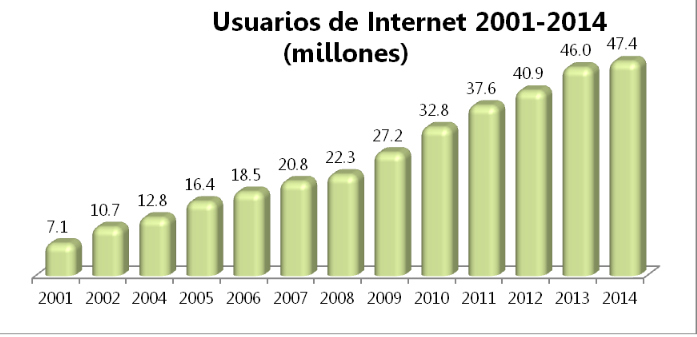
\includegraphics[width=0.7\linewidth, height=0.2\textheight]{tabla1}
\caption{}
\label{fig:tabla1}
\end{figure}

En la era del conocimiento,(como se le llama a esta decada) el acceso a Internet se encuentra asociado de manera
importante con el nivel de estudios.
De la población de cuenta con estudios de nivel superior (licenciatura o posgrado), nueve
de cada diez ha incorporado el uso de Internet en sus actividades habituales; más de dos
tercios de los que acreditaron el nivel medio superior (preparatoria o equivalente) también
lo hacen.
La siguiente grafica muestra el acceso a internet por nivel de escolaridad
\begin{figure}[h]
\centering
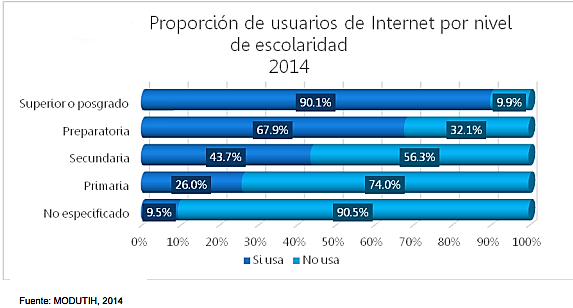
\includegraphics[width=0.7\linewidth, height=0.2\textheight]{tabla2}
\caption{}
\label{fig:tabla2}
\end{figure}

Como se logra apreciar el uso del internet va en aumento conformo los estudiantes van creciendo y adquiriendo habilidades por el uso del internet.
\newpage 
Las formas de apropiación de la información que circula, se produce y consume en el espacio socio-virtual que configura Internet, pudiendo ser agrupadas de manera tentativa en dos grandes categorías:\\
\begin{enumerate}
	\item Participando como consumidores de información producida por otros usuarios, donde el rol de consu-midor sólo implica la búsqueda y recolección de datos.\\
	\item Asumiendo un rol como partícipe directo en la elaboración de los materiales que circulan en la Red,de constructor de información y, cuando ésta es organizada y sistematizada de manera tal que logra unsignificado, constructor de conocimiento.\\
\end{enumerate}
 
En este último caso, se tratará de una contribución a partir de la creación de contenidos para ser publicados en el espacio virtual.Las formas que podrá asumir esta modalidad abarcan un continuo, que va desde la actuación como interlocutor o animador en una lista deinterés hasta diseñador y elaborador individual o colectivo de páginas en la WWW (World Wide Web)[6]\\

Una primera respuesta visible de muchas universidades se ha expresado de tres maneras:  
\begin{enumerate}
	\item Mediante la proyección de su imagen y de sus servicios a través de sitios web orientados al gran público.
	\item Mediante el desarrollo de sistemas de apoyo a su labor académica: sitios de consulta para alumnos 
	\item En algunos casos, bastante más escasos, en el desarrollo de sistemas de docencia a distancia.[10]\\
\end{enumerate}

Algunos ejemplos de proyectos y recursos creados por profesores y aprendices son:
materiales de cursos en línea, documentos administrativos en línea, material de referencia en línea, construcción de cursos que usan la red, creación de proyectos con recursos y dirección centralizada, entorno a un concepto o método, ambientes de trabajo distribuido, foros de discusión sobre curriculum, aprendizaje, metodología, tele-educación, colaboraciones completamente distribuidas, recursos compartidos, grupos locales dirigiendo sus propias actividades, marco de organización compartida, acceso a redes educativas nacionales e internacionales, construcción de recursos educacionales en red.[7]\\

También se realizan proyectos al nivel de laboratorios globales, en los cuales se desarrollan investigaciones basadas en proyectos del mundo real, que se apoyan en tecnologías avanzadas y tele-educación, y se basan en la colaboración internacional y curriculum innovador del medioambiente. [7]



\newpage
Muchas son las ventajas de trabajar con Internet en educación, las se verán incrementadas en la medida
que el profesor planifique estrategias de acción pertinentes a su grupo de aprendices, pues no se debe
olvidar que Internet es un medio y no un fin, por lo que los resultados dependen del trabajo pedagógico
que se realice utilizando Internet y ello a su vez, dependerá del uso que el facilitador y los aprendices
hagan de ella.\\

Entre las ventajas más importantes encontramos que Internet:
\begin{itemize}

\item Estimula el uso de formas nuevas y distintas de aprender/construir

\item Cuenta con buenas herramientas de apoyo al trabajo colaborativo, diseño, desarrollo y evaluación
de proyectos, investigación, experimentación y trabajo interdisciplinario.

\item Ayuda a aprender de otros y con otros.

\item Facilita el aprender haciendo, construyendo cosas y resolviendo problemas.

\item Estimula el desarrollo y uso de destrezas de colaboración, comunicación e interacción.

\item Estimula el desarrollo y uso de destrezas sociales y cognitivas.

\item Estimula el trabajo global y la interdisciplinariedad.\\ \\
\end{itemize}

Las desventajas al usar Internet en educación radican esencialmente en:
\begin{itemize}
	\item La cantidad y calidad de la información circulante

\item El tiempo que el profesor y alumno requiere para navegar

\item Las metodologías de trabajo son aún inmaduras

\item La carencia de evaluación de experiencias educativas con el uso de Internet como medio

\item La carencia de mapas visibles que permitan al usuario orientarse dentro de la información y
evitar la saturación por información diversamente representada, llamada fatiga cognitiva.
\end{itemize}
\section*{CONCLUSIÓN}
El avance de la tecnologia siempre ira de la mano de la educacion, aprender a usarlas de manera adecuada nos ayudara en un futuro a la optimizacion del tiempo de busqueda de informacion valida, tanto para estudiantes como profesores puesto que ambos se iran adaptando periodicamente al uso del internet en la realizacion de trabajos importantes.
\newpage
\section*{REFERENCIAS}
	\begin{enumerate}
		\item \textit{ Aspectos negativos del uso del internet en la educacion superior.}\\
		http://www.eumed.net/rev/ced/27/gar.htm
		\item \textit{Las nuevas culturas de aprendizaje y su incidencia en la educación superior}\\
		http://www.scielo.org.mx/scielo.php?pid=S1405-66662011000400008\&script=sci\_arttext
		
		\item  \textit{Hacia la calidad y accesibilidad en Internet}\\
		http://hdl.handle.net/10366/118799
		
		\item \textit{Las bibliotecas en la era de Internet.}\\
		http://hdl.handle.net/10366/118759
		
		\item \textit{Las dimensiones de Internet en 2012}\\
			http://mexicanadecomunicacion.com.mx/rmc/2013/04/22/las-dimensiones-de-internet-en-2012/
		\item 	 \textit{Estadisticas a proposito del dia mundial del internet}\\
			http://www.inegi.org.mx/saladeprensa/aproposito/2015/internet0.pdf
			\item 	 \textit{Usos Educativos de Internet}
			http://users.dcc.uchile.cl/~jsanchez/Pages/papers/usoseducativosdeinternet.pdf
			\item 	\textit{ Historia del internet}\\
			http://es.ccm.net/contents/229-historia-de-internet.
			\item \textit{Historia de los inicios de Internet}\\
			http://www.elpopular.pe/series/reportero-escolar/2014-05-15-historia-de-los-inicios-de-internet.
			\item 	\textit{Colle, Raymond (2003): Reflexiones sobre la universidad en la era de la información. Revista Latina de Comunicación Social, 54. Recuperado el 17 de Mayo de 2016 de:}\\
			http://www.ull.es/publicaciones/latina/200353colle.htm 
			
	\end{enumerate}   
	 

%\nocite{oreg,schn,pond,smith,marg,hunn,advi,koha,mouse}

%%%%%%%%%%%%%%%%%%%%%%%%%%%%%%%%%%%%%%%%%%%%%%
%%                                          %%
%% Backmatter begins here                   %%
%%                                          %%
%%%%%%%%%%%%%%%%%%%%%%%%%%%%%%%%%%%%%%%%%%%%%%

\begin{backmatter}






%%%%%%%%%%%%%%%%%%%%%%%%%%%%%%%%%%%%%%%%%%%%%%%%%%%%%%%%%%%%%
%%                  The Bibliography                       %%
%%                                                         %%
%%  Bmc_mathpys.bst  will be used to                       %%
%%  create a .BBL file for submission.                     %%
%%  After submission of the .TEX file,                     %%
%%  you will be prompted to submit your .BBL file.         %%
%%                                                         %%
%%                                                         %%
%%  Note that the displayed Bibliography will not          %%
%%  necessarily be rendered by Latex exactly as specified  %%
%%  in the online Instructions for Authors.                %%
%%                                                         %%
%%%%%%%%%%%%%%%%%%%%%%%%%%%%%%%%%%%%%%%%%%%%%%%%%%%%%%%%%%%%%

% if your bibliography is in bibtex format, use those commands:
%\bibliographystyle{bmc-mathphys} % Style BST file (bmc-mathphys, vancouver, spbasic).
%\bibliography{bmc_article}      % Bibliography file (usually '*.bib' )
% for author-year bibliography (bmc-mathphys or spbasic)
% a) write to bib file (bmc-mathphys only)
% @settings{label, options="nameyear"}
% b) uncomment next line
%\nocite{label}

% or include bibliography directly:
% \begin{thebibliography}
% \bibitem{b1}
% \end{thebibliography}

%%%%%%%%%%%%%%%%%%%%%%%%%%%%%%%%%%%
%%                               %%
%% Figures                       %%
%%                               %%
%% NB: this is for captions and  %%
%% Titles. All graphics must be  %%
%% submitted separately and NOT  %%
%% included in the Tex document  %%
%%                               %%
%%%%%%%%%%%%%%%%%%%%%%%%%%%%%%%%%%%

%%
%% Do not use \listoffigures as most will included as separate files







%%%%%%%%%%%%%%%%%%%%%%%%%%%%%%%%%%%
%%                               %%
%% Additional Files              %%
%%                               %%
%%%%%%%%%%%%%%%%%%%%%%%%%%%%%%%%%%%




\end{backmatter}
\end{document}
